% %%%%%%%%%%%%%%%%%%%%%%%%%%%%%%%%%%%%%%%%%%%%%%%%%%%%%%%%%%%%%%%%%%%%%%%%%%%%%%%%
%
% example.tex :
% Based on example.tex by J. Dreissig (julian.dreissig@physik.de) for GSI Summer 
% Student Program 1999.
% Recycled for the Summer Student Program in 2007 and 2008.
% 
% This Latex2e file contains an example layout for your final report.
%
%   2007:
%   Maciek Sobczak, macieksobczak@wp.pl
%   Friedemann Zenke, fzenke@gmail.com
%
%   2008:
%   04herbst@edu.uni-graz.at
%
% %%%%%%%%%%%%%%%%%%%%%%%%%%%%%%%%%%%%%%%%%%%%%%%%%%%%%%%%%%%%%%%%%%%%%%%%%%%%%%%%
% DO NOT EDIT!
% BEGIN Header
\documentclass[twocolumn,gsifonts,twoside]{gsipaper}
\usepackage{a4wide,gsiindex,helvet}
\usepackage[english]{babel}
\usepackage{amsmath,amsfonts,amssymb,verbatim,float}
\usepackage[pdftex]{graphicx} % Graphic files: pdf or jpg

\begin{document}
% END Header

% Edit below this line
% %%%%%%%%%%%%%%%%%%%%%%%%%%%%%%%%%%%%%%%%%%%%%%%%%%%%%%%%%%%%%%%%%%%%%%%%%%%%%%%%


% -= NOTA BENE =-
% Replace the title, abstract, authors, and addresses within the curly brackets
% with your own title, authors, and  addresses. You may have as many authors and
% addresses as you need.  The control sequences of author and addresses can be
% repeated as often as necessary. Footnotes in titles, adresses and the abstract
% need a special procedure and are described below.

\title{Quality Assurance of silicon sensors for CBM-STS}

\abstract{This report introduces CBM-STS detector and the Quality Test Center(QTC)
	in GSI. It also details the hardware and setup for quality assurance as well as
	the QA procedures, which includes optical and electrical inspection. The database
	framework for CBM-STS QA has been implemented using	the FairDB SQL Interface, 
	and QA data schemes would be shown in this paper. In addition, several diagrams
	extracting from measurement data are given.
	}

\shortauthor{Wu, Yitao}
\shorttitle{CBM-STS QA}

\author{Yitao Wu}            % first author
\address{University of Science and Technology of China, torrence@mail.ustc.edu.cn}

%\author{next author}                  % if you have more than one author,
%\address{next address}                % use these lines for the next one.

\maketitle
%\thispagestyle{empty}

% -= NOTA BENE =-
% Start your text with the following command. 

\section{Introduction}
The Compressed Baryonic Matter (CBM) experiment will carry out
 systematic research on the properties of nuclear matter under extreme conditions,
 in particular, at highest net baryon densities. These conditions will
 be met by colliding beams of heavy ions on targets in the energy range from
 2 to 14, eventually 45 GeV/nucleon, as they will be provided with highest
 intensities by the heavy-ion synchrotron SIS-100, and in a future stage
 by the SIS-300 machine of the Facility for Anti-proton and Ion Research
 (FAIR) at GSI, Darmstadt, Germany.\cite{ywu:jh}

%%%%%%%
% Picture - Sensor
%%%%%%%
\begin{figure}[htb]
	\centering
	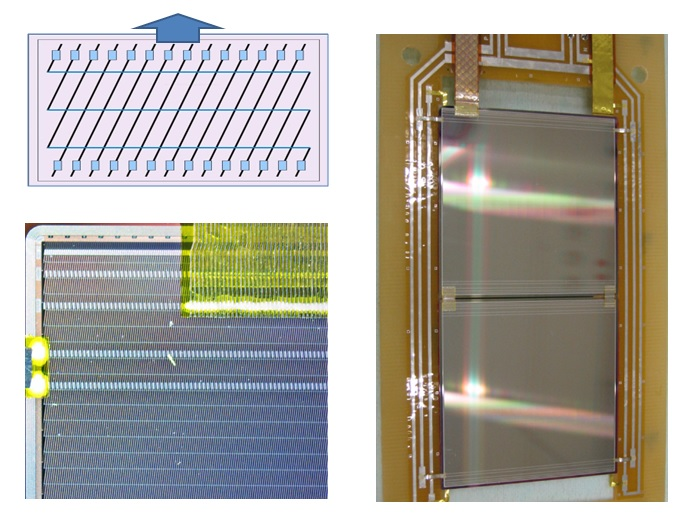
\includegraphics[width=0.45\textwidth]{fig/ywu-sensor}
	\caption{Segmentation of the micro-strip sensors (left), and prototype 
		of a read-out sector (right).}
	\label{ywu:fig:sensor}
\end{figure}

%Objective, Requirements, Design, Principle, Geometry, Readout, DAQ

The Silicon Tracking System (STS) is the central detector fo the CBM
 experiment. Its task is the standalone trajectory and momentum reconstruction
 of the high multiplicities of charged particles originating from high-rate
 beam-target interactions. The silicon microstrip detectors must be
 radiation hard and are read out by a fast self triggering front-end electronics.

The sensor technology used in STS is required to provide high track reconstruction
 efficiency as well as low material budget. As a result, the double-sided, 300 $\mu m$ thick
 microstrip sensor with a second metalization layer were chosen. The geometry design of STS
 sensor is illustrated in Fig. \ref{ywu:fig:sensor}. There are 1024 micro strips in
 each layer. Between the ''p'' and ''n'' side strip orientation of the sensor, there
 is a stereo angle of 7.5$^{\circ}$ in order to readout in one direction which reduce
 space for installation. For final design, a family of sensors will be employed, which
 are realized in four discrete sizes, $6.2\times 2.2,~6.2\times 4.2,~6.2\times 6.2$ 
 and $6.2\times 12.4~cm^{2}$.

%%%%%%%
% Picture - STS
%%%%%%%
\begin{figure}[htb]
	\centering
	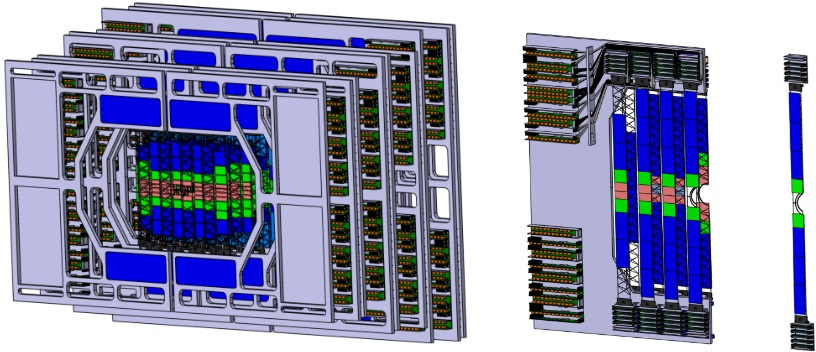
\includegraphics[width=0.45\textwidth]{fig/ywu-STS}
	\caption{Conceptual design of CBM-STS, showing the ensemble of eight
		stations with the support frame (left) and a half station with
		ladders and FEE readout (right)}
	\label{ywu:fig:sts}
\end{figure}

% Motivation program of QA. Task and condition in QTC
The STS will consist of eight planar tracking stations with about 900 readout units
 (see Fig.\ref{ywu:fig:sts}), which is comprised of sensor, micro-cable
 and FEB (front-end board).
 Once a module has been built it can not be modified or repaired.
 This is why quality assurance (QA) for every component is very important before module assembly. 
 Due to a large-scale production, the effective QA of sensors can be
 achieved by a collective effort among the Quality Test Centers, one of them is built in GSI
 cleanroom (see Fig. \ref{ywu:fig:qtc}). Fig. \ref{ywu:fig:qa} indicates the 
 variety of quality assurance tests. The
 overall QA program can be represented as a combination of tests performed on
 sensor and strip level.

%%%%%%%
% Picture - QTC
%%%%%%%
\begin{figure}[htb]
	\centering
	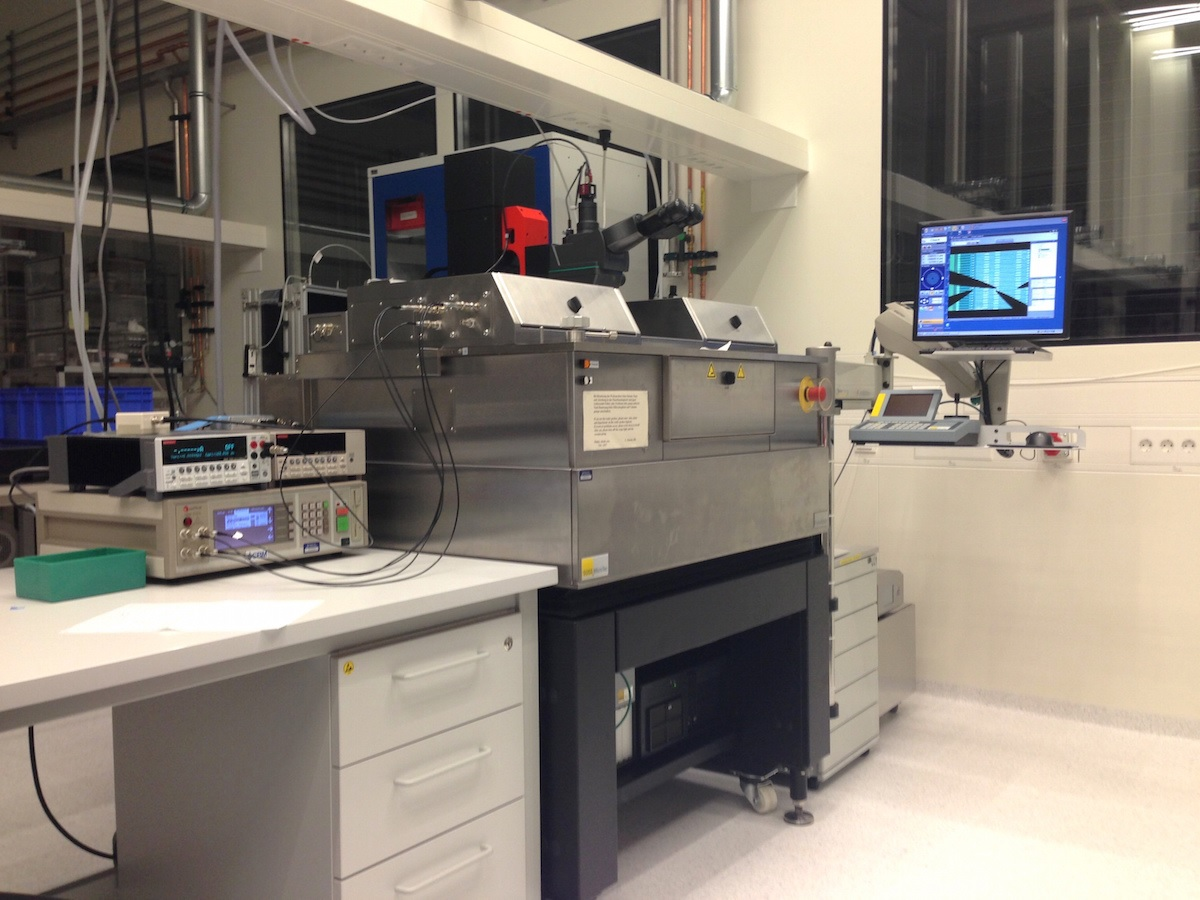
\includegraphics[width=0.45\textwidth]{fig/ywu-QTC}
	\caption{General view of the Quality Test Center (QTC) in GSI cleanroom. \cite{ywu:pl}}
	\label{ywu:fig:qtc}
\end{figure}

\section{Quality Assurance at GSI}
\label{ywu:sec:qagsi}
Quality assurance for silicon sensor includes visual tests on arrival, control and
distribution to testing centers, verification of specifications via tests and central
database for keeping track of sensor response. To be able to perform the quality assurance
program the following equipment is used:

% Testing and storage conditions, equipments and devices
\begin{itemize}
	\item S\"uss PA300PS probe station, featuring 1 $\mu m$ movement precision
	in XYZ direction and a chuck rotation option of $\pm 7.5^{\circ}$, is itself 
	equipped with a ProberBench PC hosting the GUI operating system;
	
	\item Keithley 2410 SourceMeter unit (SMU) providing high-voltage up to
	$\pm$ 1100 V and current resolution of 10 pA;
	
	\item Keithley 6487 picoammeter/voltage source having a 2 nA - 20 mA current
	range and a high-resolution voltage source up to 505 V;
	
	\item QuadTech 7600 precision LCR-meter with customized external biasing up to
	500 V, wide frequency range from 100 Hz to 2 MHz, 0.05 \% measurement
	accuracy, programmable test voltage and current;
	
	\item Keithley 708B switching matrix (multiplexer) mainframe with a high-voltage
	(up to 1100 V) switching card (Keithley 7072-HV) for automation of the
	measurements (discussed in Chapter 5).
\end{itemize}

All the equipments for characterization has to be installed in a clean room with
 temperature $21\pm 2^{\circ}C$ and humidity control. The clean room is ISO 4 or
 better. Access to the testing area has to be limited. Protective clothing, masks
 and gloves must be worn by all personnel who handle sensors. The QA procedures
 which would be performed in clean room is listed as below:

%%%%%%%
% Picture - QA procedures
%%%%%%%
\begin{figure}[htb]
	\centering
	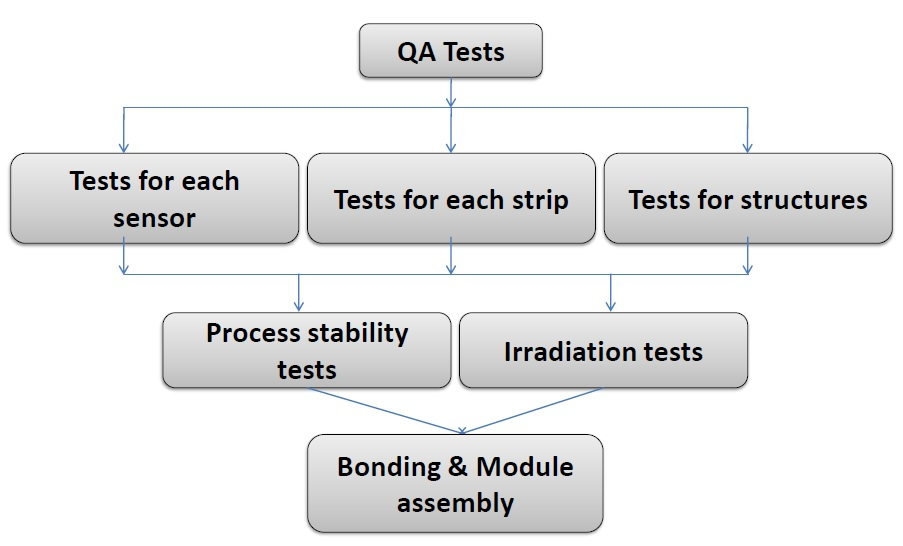
\includegraphics[width=0.45\textwidth]{fig/ywu-qa}
	\caption{Quality assurance procedures in GSI}
	\label{ywu:fig:qa}
\end{figure}

\paragraph{Bulk electrical tests} are performed to determine the overall
sensor behavior at the operational conditions. Current-voltage (I-V) and
capacitance-voltage (C-V) tests are conducted after optical inspection. The
I-V tests determines the leakage current of a sensor while the C-V tests
determines the full depletion voltage of a sensor.

\paragraph{Long-term stability tests} will be performed on a fraction of the
sensors. The leakage current of the sensors will be monitored for a time period
of 48-72 hours in order to evaluate their stability.

\paragraph{Strip diagnostic tests} aim to identify strip defects originating
from the complex fabrication process that cannot be identified by the optical
inspection. These defects comprise mainly ohmic contacts or short circuits
between the strip implant and the readout strip (so-called ``pinholes''), short
circuits between two or more readout strips, and strips exhibiting high leakage
current. As shown in Fig. \ref{ywu:fig:needle}, probe needle 1 contacts with DC pad
of the middle strip, and needle 2, 3, 4 contacts AC pads of neighboring strip respectively.
In such setup, we could measure all the necessary parameters for strip test which
are also listed in Tab. \ref{ywu:table:strip}. Strip leakage current can be measured
with needle 1 directly. With needle 1 and 3, we can measured pinhole and coupling capacitance.
The needle 2 or 4 should be used to test the short circuit between aluminum readout and silicon strip,
 incorporated with needle 3.  

%%%%%%%
% Picture - Probe needle setup
%%%%%%%
\begin{figure}[htb]
	\centering
	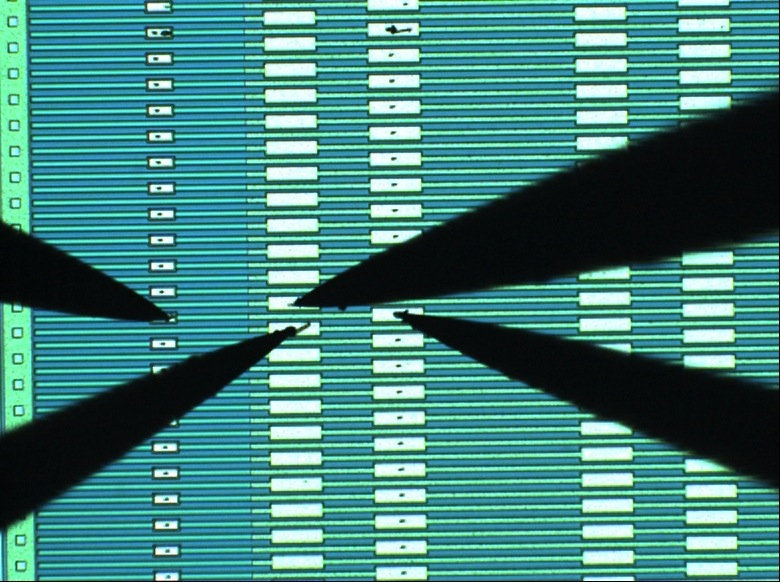
\includegraphics[width=0.45\textwidth]{fig/ywu-needle}
	\caption{Arrangement of the instruments for a multi-purpose strip diagnostic
		test. Four probe needles contacts the neighboring AC or DC pads. \cite{ywu:pl}}
	\label{ywu:fig:needle}
\end{figure}

Fig. \ref{ywu:fig:pinhole} shows the pinhole test result
of all the strip in a sensor's one side. It demonstrate that results in lab can vary from
that provided by the producer because defects can develop during storage and transportation. 

%%%%%%%
% Picture - Result extracted from database, Pinhole
%%%%%%%
\begin{figure}[htb]
	\centering
	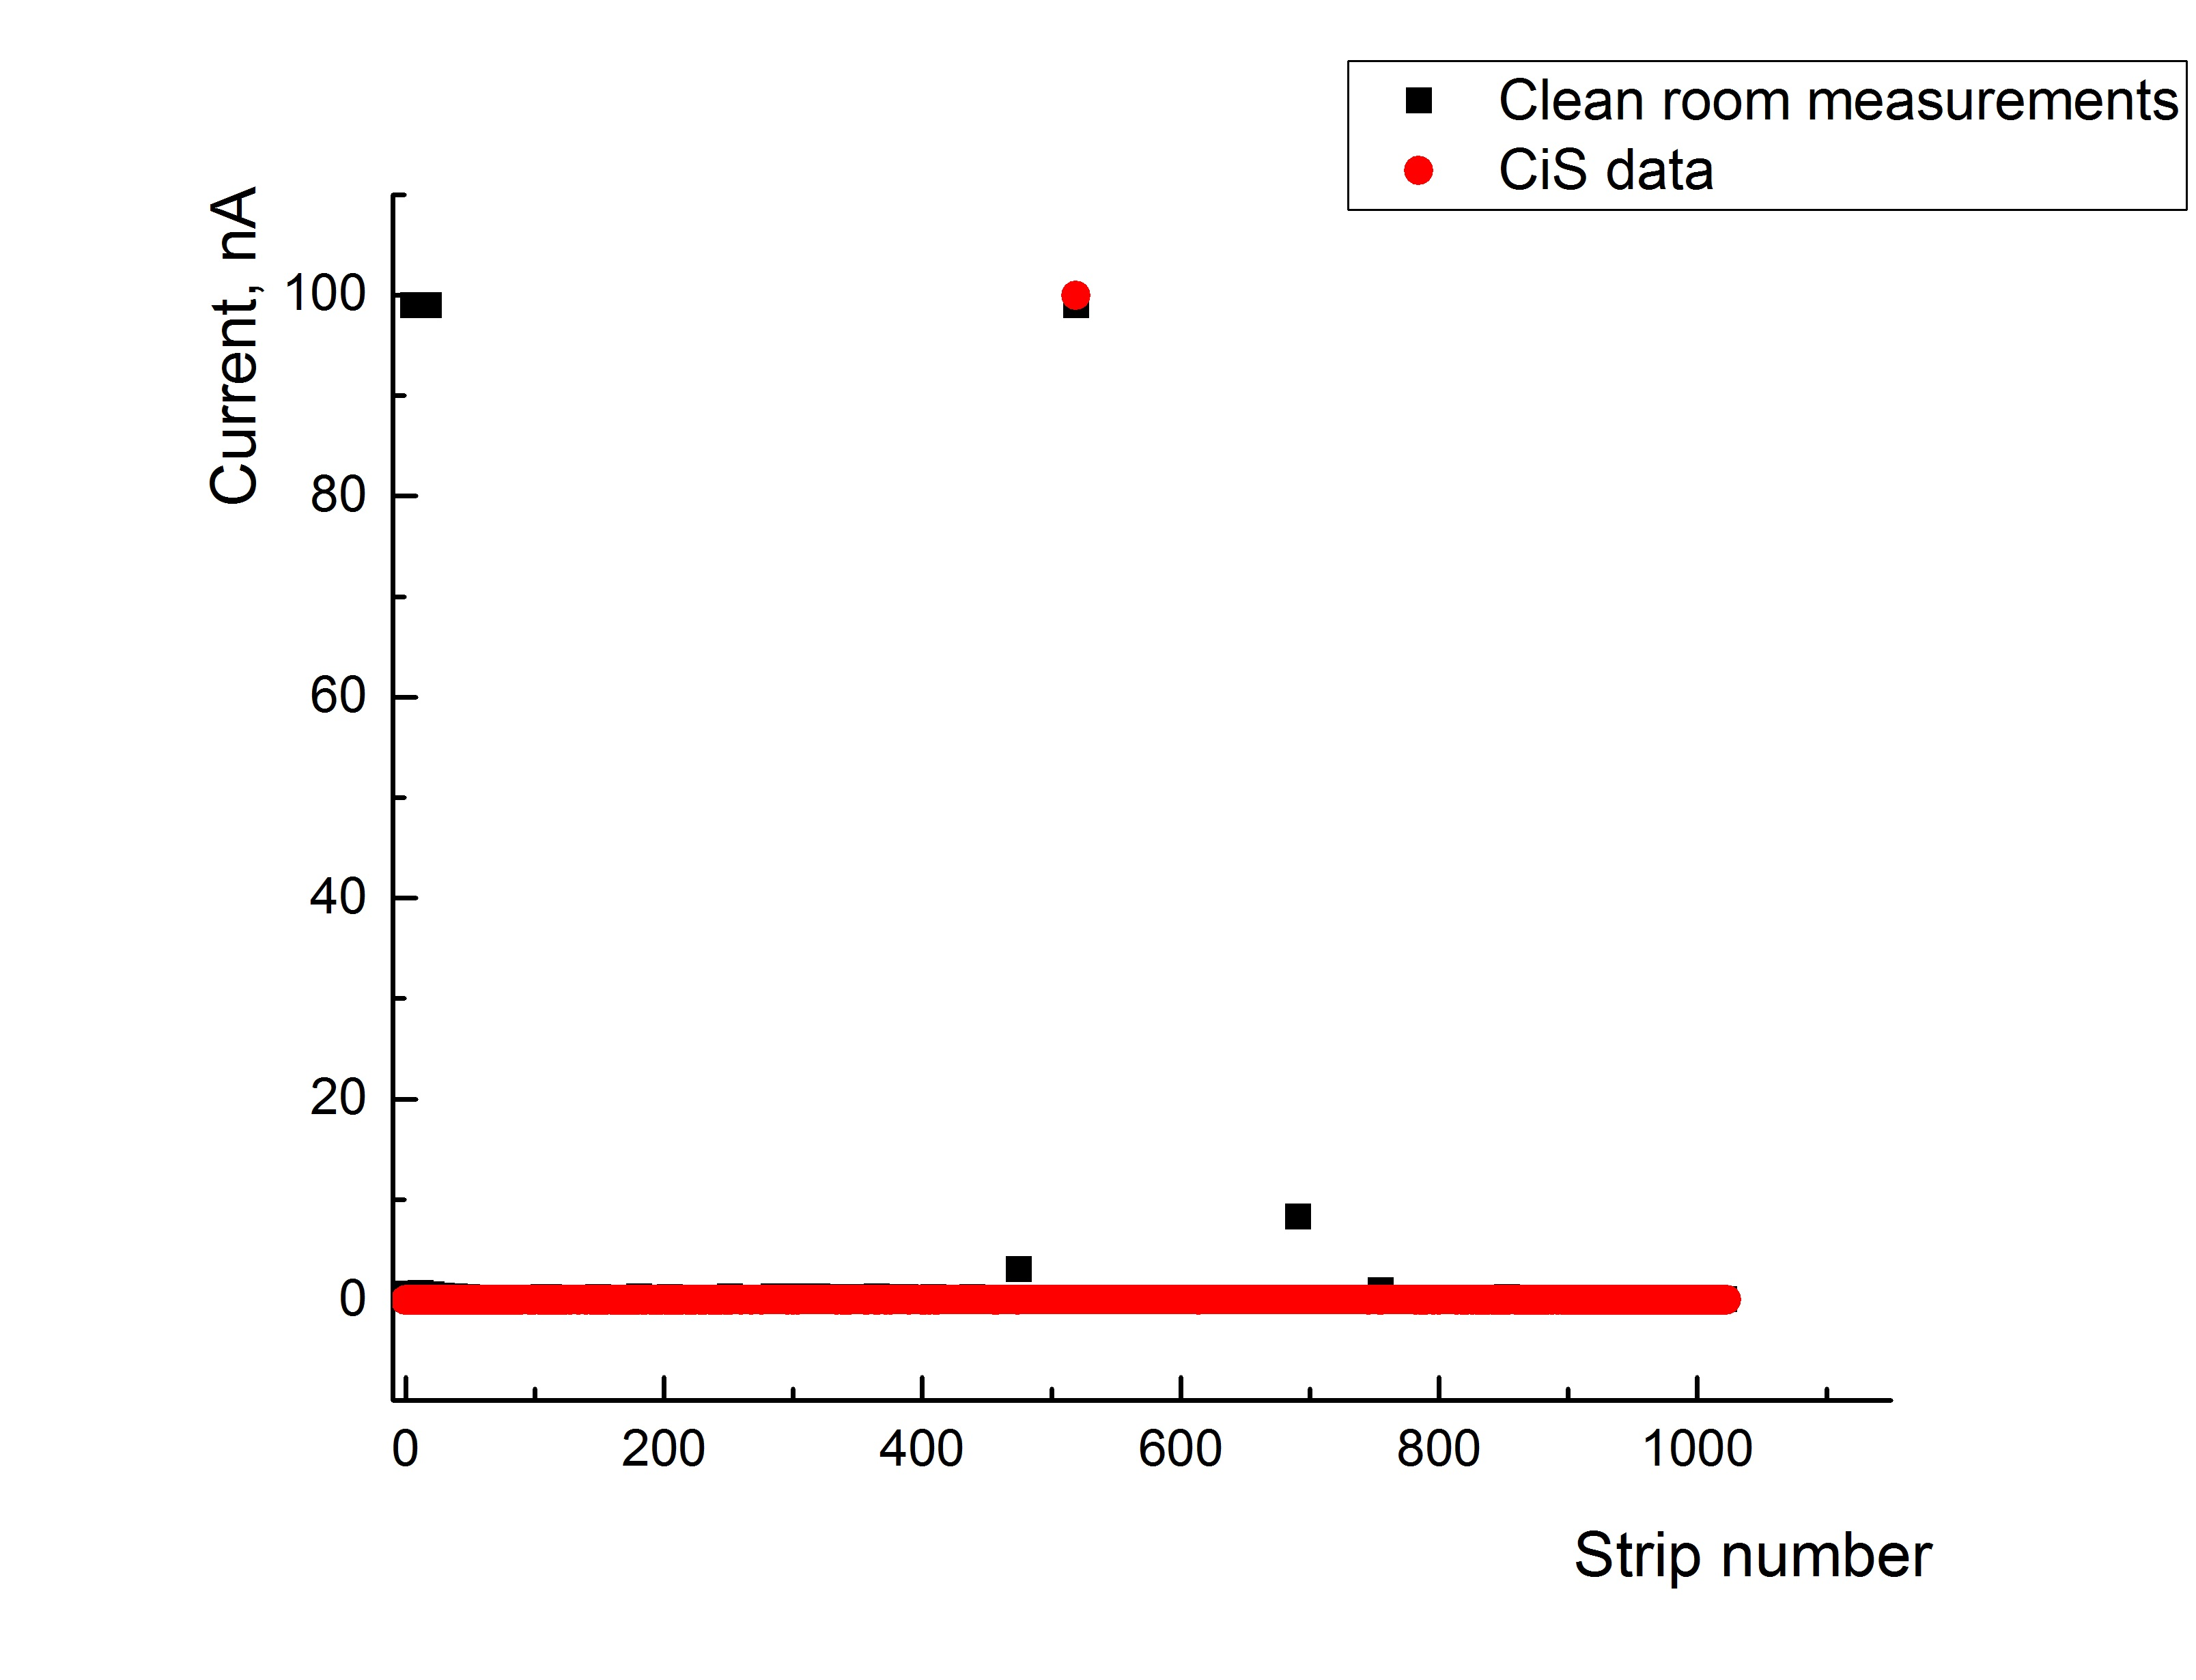
\includegraphics[width=0.45\textwidth]{fig/ywu-pinhole}
	\caption{Pinhole scan of silicon microstrips, result extracted from database.}
	\label{ywu:fig:pinhole}
\end{figure}

\section{QA Database}
An important part of the QA is the availability of all information concerning the sensors.
 This includes not only test results form optical and electrical QA, but also information
 on ordering and delivery of the sensors. In addition, the QA centers will keep track of
 sensors which do not, or only partly, meet the specifications.

The CBM STS quality assurance (QA) database will gather into one repository all relevant
 measurements obtained during the STS sensors tests performed by the STS QA responsible
 laboratories. Any new or updated results will be stored in a dedicated database and can
 then be directly accessed form any location either a web interface or ROOT macro.

A central database is also important for tracking the shipment of sensors and other
 components between institutions during their lifetime. The FairDB data scheme contains,
 among others, the tables and structures for these logistic purpose.   

%%%%%%%
% Picture - CBM STS data scheme
%%%%%%%
\begin{figure}[htb]
	\centering
	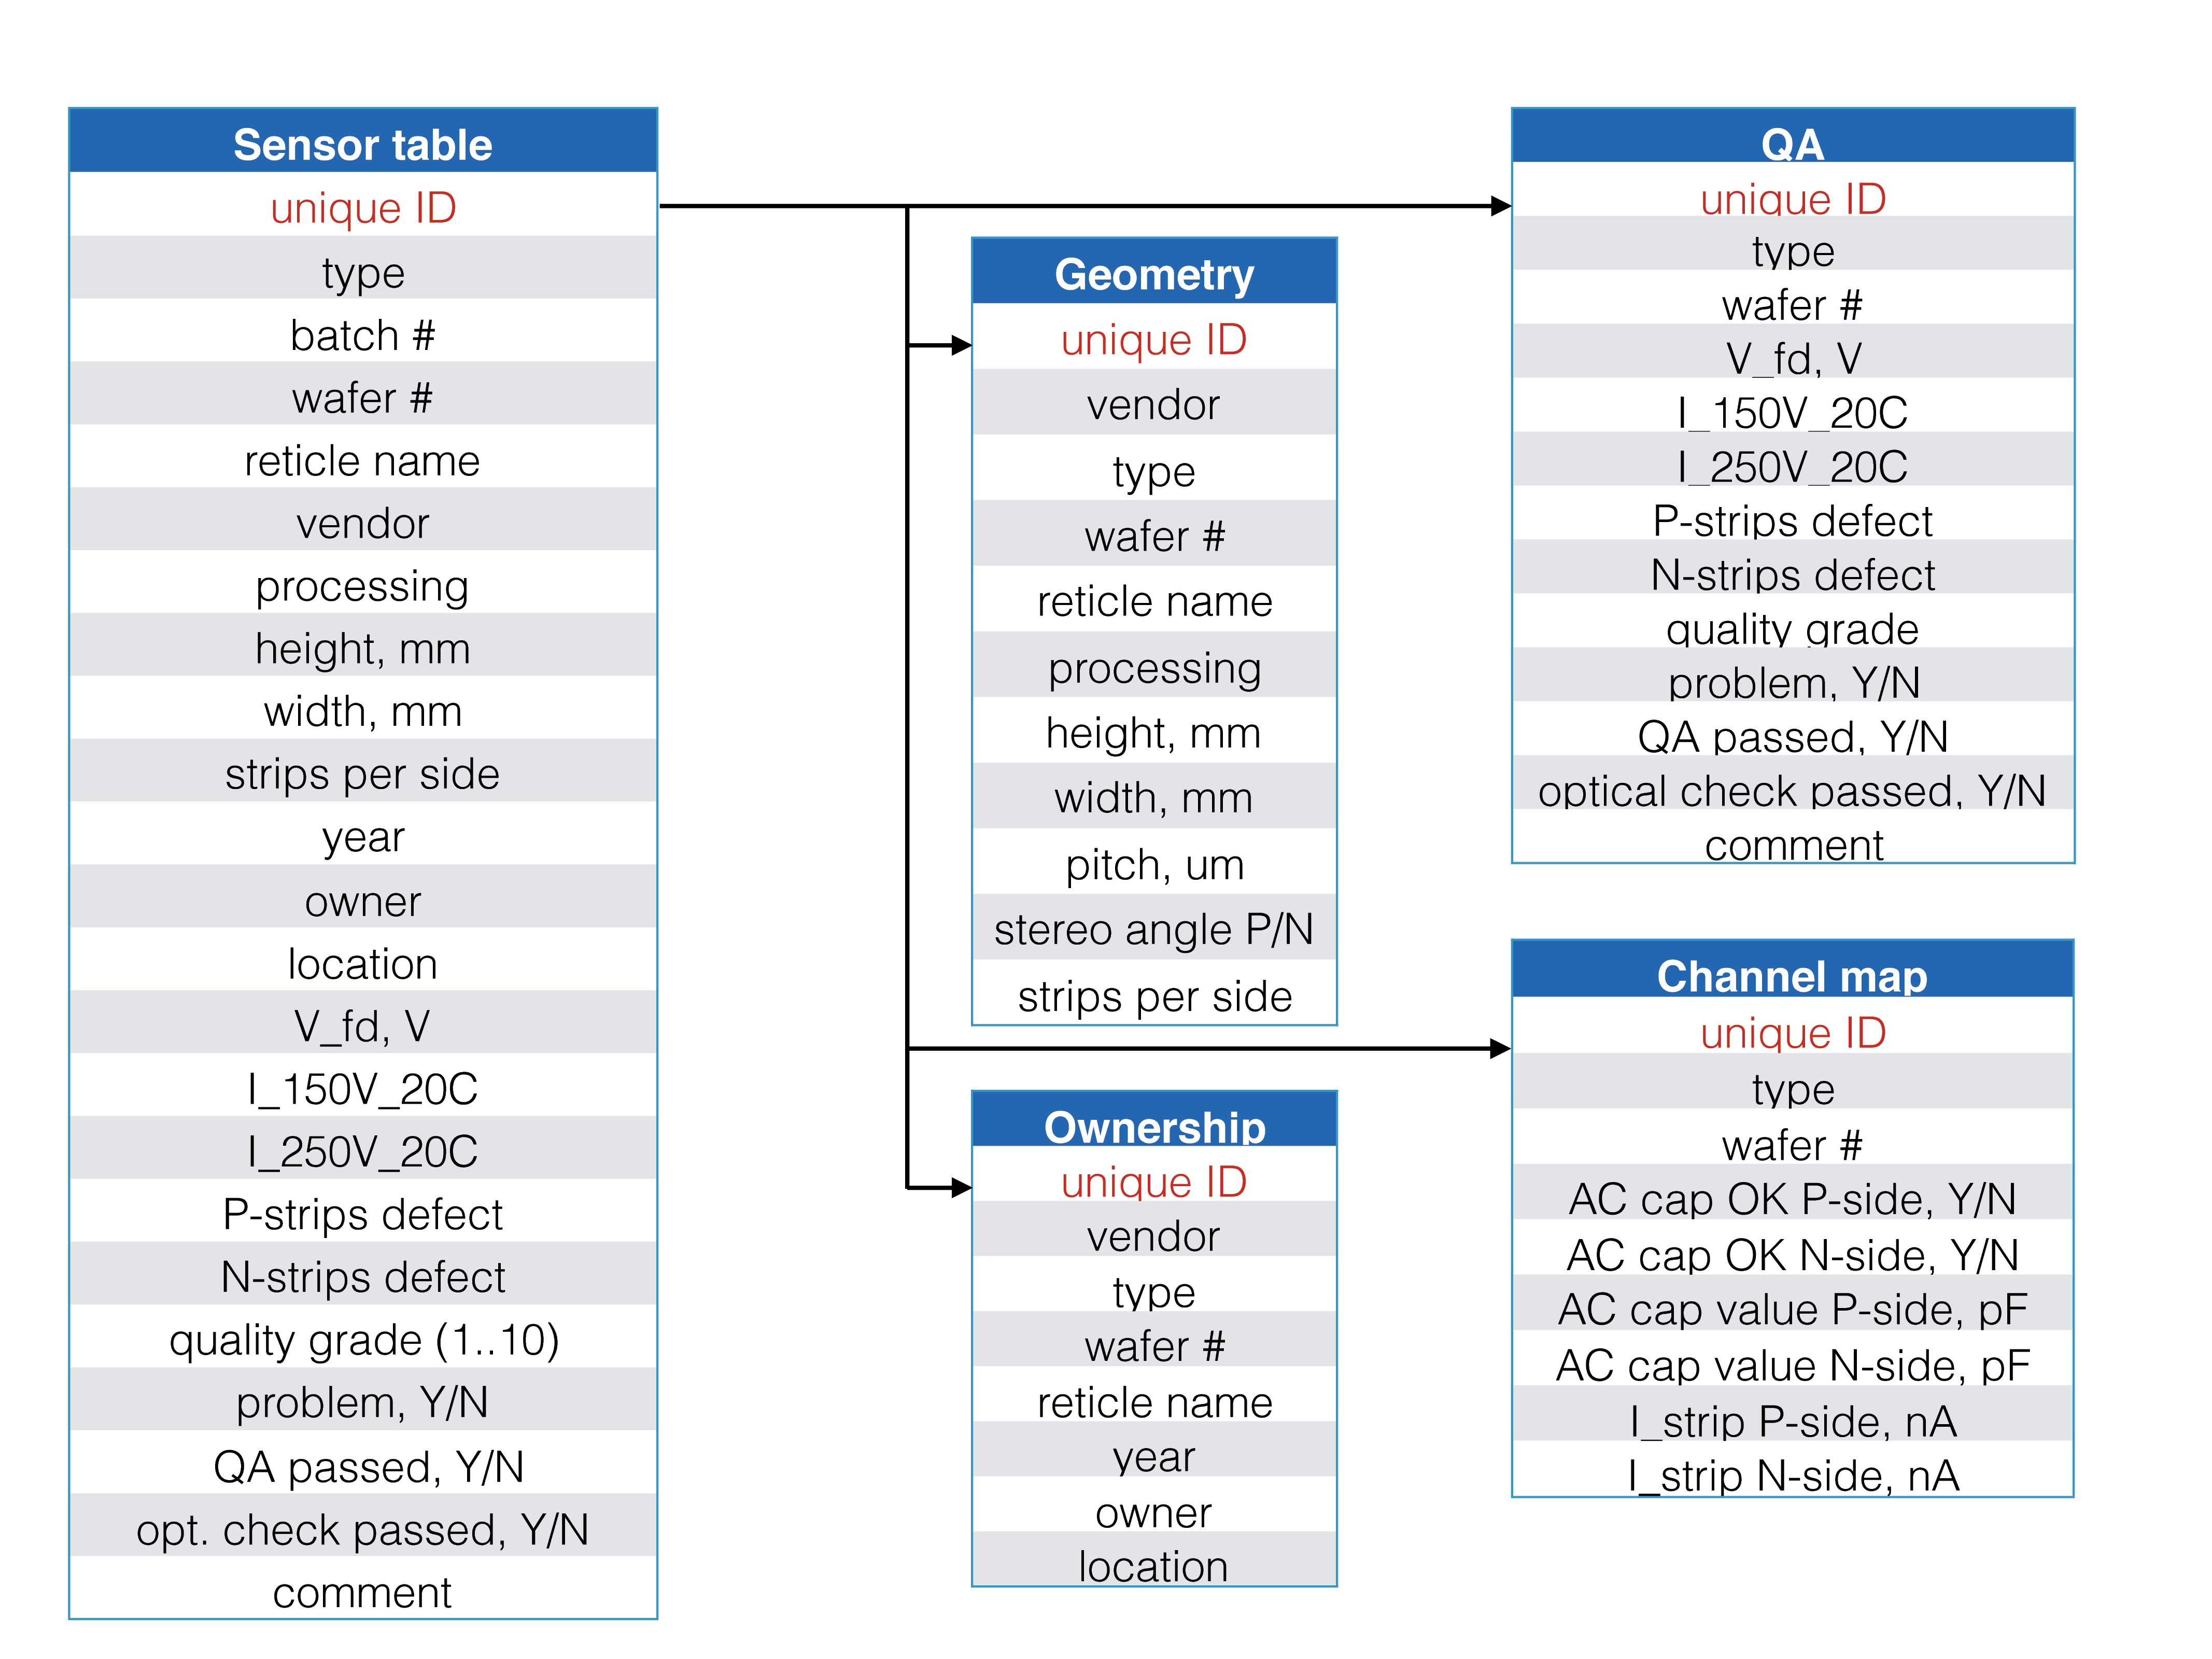
\includegraphics[width=0.45\textwidth]{fig/ywu-stsdb}
	\caption{Quality assurance data scheme. \cite{ywu:ob}}
	\label{ywu:fig:stsdb}
\end{figure}

\subsection{Design}
All new STS QA measurements as well as their history should be recorded. For this
 purpose the STS QA database is implemented using FairDB based on ROOT Library.

The FairDB will be used to store a large number of sensor parameters. These information
is used to make decision on defect severity in order to accept or reject a sensor under
test for future use in STS detector.

A main sensor table is mapped to a ROOT based QA parameter manager which holds
 different lists of sensor features indexed via the sensor unique ID (see 
 Fig. \ref{ywu:fig:stsdb}). The feature include sensor geometry, ownership, channel
 map and QA results \cite{ywu:ob}. 

%%%%%%%%
% Table - Data scheme for strip test
%%%%%%%%
\begin{table}[t]
	\centering
	\begin{tabular}{|c|p{100pt}|}
		\hline
		\textbf{Strip table} & \textbf{Description} \\
		
		\hline
		unique ID    & Generated with sensor info\\
		
		\hline
		edge & P or N side\\
		
		\hline
		strip ID & Numbering by rule, short strips included \\
		
		\hline
		I\_strip, A & Strip leakage current \\
		
		\hline
		pinhole, A & Current between implant and aluminum readout line\\
		
		\hline
		Al\_Short\_L, A & Current between this and its neighboring left strips\\
		
		\hline
		Al\_Short\_R, A & Current between this and its neighboring right strips \\
		
		\hline
		CCoupling\_Cp, F & Capacitance between AC and DC pad \\
		
		\hline
		CCoupling\_DF, F & Deflection factor between AC and DC pad \\
		
		\hline
		Passed, Boolean & Check parameters with acceptance criteria.\\
		
		\hline
	\end{tabular}
	\caption{Strip test data scheme}
	\label{ywu:table:strip} 
\end{table}

\section{Implementation of Strip Test Table}
An implementation of the STS QA database table for strip test based on FairDB is available
 now. It stores information on sensor parameters and quality assurance results as well as
 tracking information for logistic purpose.
 
My task was to implement the database table for strip diagnostic tests. In current work,
 the information on identified defect will be stored, which
 was shown in Tab. \ref{ywu:table:strip}. All parameter classed are compatible with the
 FairDB framework scheme and could be used for the data analysis.

In order to extract the information on the strip
 properties, strip diagnostic tests will be performed. All of the parameters could be
 measured using probe station and devices in cleanroom (see Sect. \ref{ywu:sec:qagsi}).
 

\section{Summary}
In the two months study in GSI CBM-STS group, I have visited the lab and cleanroom in
 GSI, where my tutors showed me how to perform QA procedures with those professional
 equipments and devices. Then it takes me a lot of time to understand the design, principle
 and readout method of the silicon sensor. Furthermore, in order to take advantage of 
 the measurements data and extract more useful information, I have took a brief tutorial 
 about FairDB. With a fully configure STS database server,  I could practice all the 
 operations and interfaces provided which helps me a lot to get familiar with FairDB. 
 
\section*{Acknowledgments}
I would like to express my gratitude to my tutor Olga Bertini and Anton Lymanets for given
 possibility to work on such important and interesting project. Then I thanks to the GSI
 CBM-STS group members for their assistance and parties during the program. Special sincerely 
 thanks to J{\"o}rn Knoll and all the GSI persons who contributed to ISSP. In the end, I really 
 benefit a lot from this experience, thanks to all the students who contributed to and 
 participated in such memorable summer.

%Maksym Teklishyn, Hanna Malygina, Adrian Rodriguez Rodriguez, Ievgeniia Momot;

\begin{thebibliography}{99}

%\cite{Heuser:2016coc}
\bibitem{ywu:jh} 
J.~M.~Heuser [CBM Collaboration], \textsl{Status of the Compressed Baryonic Matter
	Experiment at FAIR and Its Silicon Tracking System},
Acta Phys.\ Polon.\ Supp.\  {\bf 9}, 221 (2016).
%%CITATION = doi:10.5506/APhysPolBSupp.9.221;%%

\bibitem{ywu:pl}
P. Larionov, \textsl{Systematic Irradiation Studies and Quality Assurance of
Silicon Strip Sensors for the CBM Silicon Tracking System}, PhD thesis, Johann
Wolfgang Goethe-Universit{\"a}t in Frankfurt am Main, 2016.

\bibitem{ywu:ob}
O. Bertini etc., \textsl{Specifications for Quality Assurance of Microstrip
	Sensors in the CBM Silicon Tracking System}, STS Note 2016-1, 2016

\bibitem{ywu:db}
D. Bertini. \textsl{FairRoot Virtual Database (User Manual)}. 2013

\end{thebibliography}

% %%%%%%%%%%%%%%%%%%%%%%%%%%%%%%%%%%%%%%%%%%%%%%%%%%%%%%%%%%%%%%%%%%%%%%%%%%%%%%%%
% Do NOT edit below this line
% %%%%%%%%%%%%%%%%%%%%%%%%%%%%%%%%%%%%%%%%%%%%%%%%%%%%%%%%%%%%%%%%%%%%%%%%%%%%%%%%

\end{document}

% %%%%%%%%%%%%% END OF example.tex %%%%%%%%%%%%%%%%%%%%%%%%%%%%%%%%%%%%%%%%%%%%%%%